\section{Methodology（方法）}
\label{sec:method}

\subsection{Problem formulation（问题描述）}
\label{sec:problem}

考虑参数 $\mu\in\mathcal P\subset\mathbb R^d$ 控制的二维稳态对流传热问题。速度、压力与温度满足不可压缩流动的质量、动量守恒方程与能量方程；流动可以由浮力、壁面运动或进口流量驱动，也可以是给定的速度场。参数可以是 Rayleigh、Prandtl、P\'eclet 数等无量纲参数，也可以是几何尺寸。几何参数经映射 $\Omega(\mu)=\mathcal T_\mu(\hat\Omega)$ 转到固定的参考域 $\hat\Omega$，网格在 $\hat\Omega$ 上固定，各参数点的离散解向量逐分量对应。关心的传热量为壁面局部与平均 Nusselt 数、壁温等，都是解的泛函。

每个参数点上，高保真离散给出一个大规模代数方程组，一般为非线性。设计与参数分析需要在 $\mathcal P$ 内的大量参数点上求解。参数化降阶以少量训练参数点上的高保真解构造低维模型，在任意查询参数处求近似解。本文所用算例的参数、边界条件与离散见第~\ref{sec:setup} 节与\ref{app:cases}。

\subsection{Projection-based reduced-order model and base space（投影降阶与基础空间）}
\label{sec:base}

高保真离散的未知量分为主场 $\mathbf q\in\mathbb R^n$ 与辅助场 $\mathbf z$，稳态离散方程记为 $F(\mathbf q,\mathbf z;\mu)=\mathbf 0$ 与 $H(\mathbf q,\mathbf z;\mu)=\mathbf 0$。主场取容许坐标：非齐次边界值由一个与参数无关的提升承担，任意 $\mathbf q$ 加上提升后都满足主场的边界条件与离散约束。降阶只作用于主场；辅助场保留在全阶离散上，给定 $\mathbf q$ 由 $H=\mathbf 0$ 解得 $\mathbf z=\mathcal S_\mu(\mathbf q)$。代回主场方程，得到有效残差及其雅可比：
\begin{equation}
r_{\mathrm{eff}}(\mathbf q;\mu)=F\big(\mathbf q,\mathcal S_\mu(\mathbf q);\mu\big),\qquad
J_{\mathrm{eff}}=\frac{\partial F}{\partial\mathbf q}-\frac{\partial F}{\partial\mathbf z}\Big(\frac{\partial H}{\partial\mathbf z}\Big)^{-1}\frac{\partial H}{\partial\mathbf q}.
\label{eq:reff}
\end{equation}
没有辅助场时，$r_{\mathrm{eff}}=F$，$J_{\mathrm{eff}}=\partial F/\partial\mathbf q$。主场的内积 $\langle\mathbf a,\mathbf b\rangle_M=\mathbf a^{\mathsf T}M\mathbf b$ 由对称正定矩阵 $M$ 给出，POD、正交化、网络训练与误差评价都使用这一度量；$P_X=XX^{\mathsf T}M$ 为到 $M$ 正交基 $X$ 所张空间的投影。

投影降阶在仿射试探空间 $\bar{\mathbf q}+\operatorname{span}X$ 中近似主场，降阶解由有效残差在该空间上的 Galerkin 投影确定：
\begin{equation}
\mathbf q_r(\mathbf c)=\bar{\mathbf q}+X\mathbf c,\qquad
\mathbf g(\mathbf c;\mu)=X^{\mathsf T}\,r_{\mathrm{eff}}\big(\mathbf q_r(\mathbf c);\mu\big)=\mathbf 0 .
\label{eq:galerkin}
\end{equation}
求解该方程需要在任意降阶状态上计算高保真离散的有效残差与雅可比，辅助场随之在全阶离散上更新；因此快照、参考解与降阶求解都基于同一套离散。有效残差对 $\mathbf q$ 线性时，式~\eqref{eq:galerkin} 为线性方程组，直接求解；非线性时用 Levenberg--Marquardt 法求解（\ref{app:closure}）。

训练参数 $\{\mu_i\}_{i=1}^{N_s}$ 上的快照 $\mathbf q_i$（均值 $\bar{\mathbf q}$）在 $M$ 内积下作 POD~\cite{sirovich1987turbulence,berkooz1993proper}，保留相对奇异值大于 $\delta_V$ 的方向，得到 POD 基 $V$；在式~\eqref{eq:galerkin} 中取 $X=V$ 即 POD--Galerkin 方法。$V$ 只包含训练快照的组合，快照稀疏时，查询参数处的解中有较多成分落在 $\operatorname{span}V$ 之外。

灵敏度增广在快照之外加入解对参数的一阶变化~\cite{hay2009local}。参数经线性缩放得到坐标 $\eta(\mu)$，训练区映到 $[-1,1]^d$。每个训练点上，解对 $\eta$ 的稳态灵敏度由同一离散的雅可比求得；灵敏度正交化并去除 $V$ 的分量后，保留奇异值大于 $\tau$ 的方向得到 $S$。基础空间为
\begin{equation}
\mathbf s_{ij}=-J_{\mathrm{eff}}^{-1}\,\frac{\partial r_{\mathrm{eff}}}{\partial\eta_j}\bigg|_{(\mathbf q_i,\mu_i)},\qquad
W=[V,\ S],\qquad W^{\mathsf T}MW=I .
\label{eq:sensitivity}
\end{equation}
在式~\eqref{eq:galerkin} 中取 $X=W$ 即灵敏度增广 POD--Galerkin 方法（SA-PODG）。$W$ 包含训练快照及其一阶参数变化，与查询参数无关；本文在每个训练点都计算灵敏度，结果中的 SA-PODG 均指这一配置。

\subsection{Value-supervised neural candidate fields（场值监督的神经候选场）}
\label{sec:network}

网络以空间坐标与参数坐标 $(\mathbf x,\eta)$ 为输入，主干输出 $m$ 个原始场 $\chi_{\theta,k}(\mathbf x;\eta)$，读出分支输出系数 $w_\theta(\eta)\in\mathbb R^m$。原始场经容许映射 $\mathcal A_h$ 进入主场的容许坐标，得到候选场与网络预测：
\begin{equation}
\begin{gathered}
\Phi_\theta(\eta)=\big[\mathcal A_h\chi_{\theta,1},\ \ldots,\ \mathcal A_h\chi_{\theta,m}\big]\in\mathbb R^{n\times m},\\
\hat{\mathbf q}_\theta(\eta)=\Phi_\theta(\eta)\,w_\theta(\eta),\qquad
w_\theta=e^{\ell_\theta}\,r_\theta ,
\end{gathered}
\label{eq:candidates}
\end{equation}
其中 $\ell_\theta$ 为标量幅值分支，$r_\theta$ 为读出向量。网络只用训练快照的场值监督：
\begin{equation}
\mathcal L(\theta)=\frac1{N_s}\sum_{i=1}^{N_s}\frac{\Vert\hat{\mathbf q}_\theta(\eta_i)-\mathbf q_i\Vert_M^2}{\Vert\mathbf q_i\Vert_M^2},
\label{eq:loss}
\end{equation}
相对误差使范数相差很大的各训练点权重相当；训练过程见\ref{app:training}，灵敏度不参与训练。

候选场与训练的联系由读出层给出。$r_\theta$ 的最后一层为仿射层 $r_\theta=K\,h_\theta+\mathbf b$，固定其余参数时
\begin{equation}
\frac{\partial\hat{\mathbf q}_\theta(\eta)}{\partial\mathbf b}=e^{\ell_\theta(\eta)}\,\Phi_\theta(\eta).
\label{eq:bias}
\end{equation}
由于 $e^{\ell_\theta}>0$，$\operatorname{span}\Phi_\theta(\eta)$ 就是网络在 $\eta$ 处经读出偏置可到达的输出变化空间，网络预测 $\hat{\mathbf q}_\theta(\eta)$ 本身也在其中。NE-PODG 用这一空间提供增广方向，不直接以 $\hat{\mathbf q}_\theta$ 作为解。

\subsection{Complementary space construction and Galerkin closure（互补空间构造与 Galerkin 闭合）}
\label{sec:closure}

给定查询参数 $\mu$（坐标 $\eta$），先求候选空间的 $M$ 正交基 $Q_E=\operatorname{orth}_M\Phi_\theta(\eta)$，以相对奇异值阈值 $\delta_E$ 判定数值秩；再去除 $W$ 的分量，在 $M$ 度量下作奇异值分解，保留 $s_j>\tau$ 的方向，得到神经互补空间（图~\ref{fig:framework}）：
\begin{equation}
(I-P_W)\,Q_E=\tilde Z\,\operatorname{diag}(s_j)\,Y^{\mathsf T},\qquad
Z_\theta(\eta)=\tilde Z_{[:,\,s_j>\tau]},\qquad W^{\mathsf T}MZ_\theta=0 .
\label{eq:complement}
\end{equation}
$s_j\in[0,1]$ 只取决于 $\operatorname{span}\Phi_\theta(\eta)$ 与 $\operatorname{span}W$，表示候选方向相对 $W$ 的正交程度。增广基 $\Psi_\theta(\eta)=[W,\ Z_\theta(\eta)]$ 是 $M$ 正交的；NE-PODG 在式~\eqref{eq:galerkin} 中取 $X=\Psi_\theta(\eta)$，即在 $\bar{\mathbf q}+\operatorname{span}\Psi_\theta(\eta)$ 上求解同一 Galerkin 方程。网络只提供试探空间的方向，降阶解由控制方程确定。POD--Galerkin、SA-PODG 与 NE-PODG 的试探空间依次为 $V\subset W\subset\Psi_\theta(\eta)$，其余完全相同。

\begin{figure}[H]
\centering
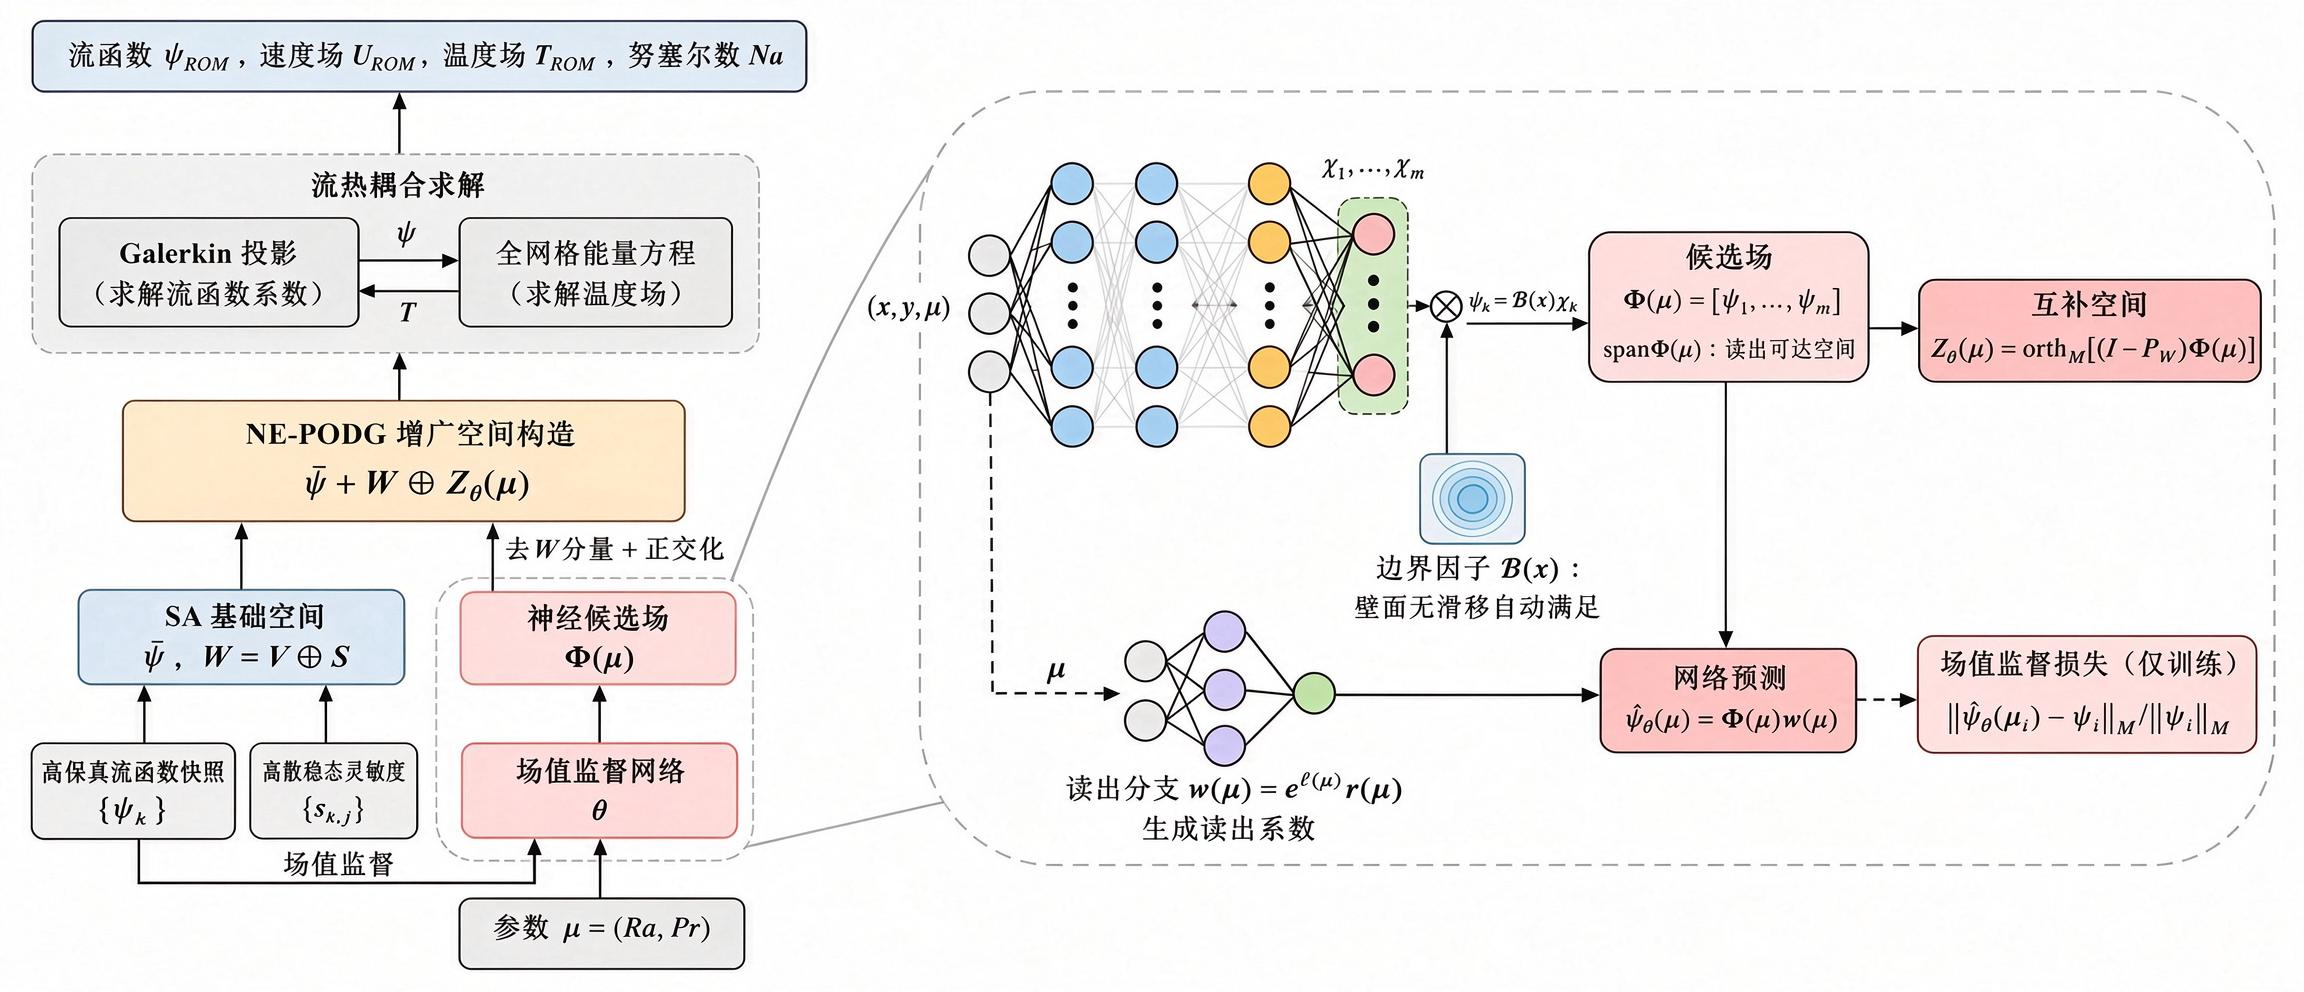
\includegraphics[width=\textwidth]{Fig_02.jpg}
\caption{NE-PODG 的总体框架。}
\label{fig:framework}
\end{figure}

\subsection{Approximation and error characterization（逼近与误差刻画）}
\label{sec:errors}

记高保真解为 $\mathbf q^\star$。对试探空间 $X\in\{V,W,\Psi_\theta\}$（增广空间上的量记下标 $B$），降阶解 $\mathbf q_X$ 的误差、最佳逼近误差与闭合放大系数为
\begin{equation}
e_X=\frac{\Vert\mathbf q_X-\mathbf q^\star\Vert_M}{\Vert\mathbf q^\star\Vert_M},\quad
e_{\mathrm{proj},X}=\min_{\mathbf q\in\bar{\mathbf q}+\operatorname{span}X}\frac{\Vert\mathbf q-\mathbf q^\star\Vert_M}{\Vert\mathbf q^\star\Vert_M},\quad
\chi_X=\frac{e_X}{e_{\mathrm{proj},X}}\ge1 .
\label{eq:errors}
\end{equation}
$\chi_X$ 衡量 Galerkin 闭合偏离最佳逼近的程度。记基础空间未表示的解余量为 $\mathbf r_W=(I-P_W)(\mathbf q^\star-\bar{\mathbf q})$，神经互补空间对它的捕获率为 $\Gamma_\theta=\Vert P_{Z_\theta}\mathbf r_W\Vert_M^2/\Vert\mathbf r_W\Vert_M^2\in[0,1]$。由于 $W$ 与 $Z_\theta$ 在 $M$ 下正交，$P_{\Psi_\theta}=P_W+P_{Z_\theta}$，于是
\begin{equation}
e_{\mathrm{proj},B}=e_{\mathrm{proj},W}\sqrt{1-\Gamma_\theta},\qquad
\frac{e_B}{e_W}=\frac{\chi_B}{\chi_W}\sqrt{1-\Gamma_\theta}.
\label{eq:error_ratio}
\end{equation}
第一式说明增广对最佳逼近误差的改善完全由 $\Gamma_\theta$ 决定。第二式将神经增广的求解误差收益分解为互补空间的余量捕获与 Galerkin 闭合放大两个因素，第~\ref{sec:mechanism} 节据此分析 NE-PODG 的精度来源。

\subsection{Benchmark problems and numerical settings（算例与数值设置）}
\label{sec:setup}

\paragraph{算例}
本文在两个参数化稳态传热问题上验证 NE-PODG（图~\ref{fig:cases}，表~\ref{tab:cases}）。方腔自然对流~\cite{devahldavis1983natural}：方腔左壁冷、右壁热，上下壁绝热，流动由浮力驱动，采用 Boussinesq 近似；参数为 $\mu=(Ra,Pr)$，速度与温度双向耦合，离散方程非线性；传热量为冷壁平均 Nusselt 数 $\overline{Nu}$。Couette--Graetz 问题取 Quarteroni 等~\cite{quarteroni2011certified}的配置：宽度为 1 的二维通道中给定 Couette 速度剖面 $u=y$，长度为 1 的入口段底壁绝热，其后长度为 $L$ 的受热段底壁施加单位热流，入口与顶壁温度为 0；参数为 $\mu=(L,Pe)$，能量方程对温度线性，对流扩散算子非对称，受热段长度经分段线性映射转到固定参考域；传热量为受热段平均壁温 $T_{\mathrm{av}}$ 与受热壁局部 Nusselt 数。两个算例的控制方程、边界条件与传热量定义见\ref{app:nc} 与\ref{app:graetz}。

\begin{figure}[H]
\centering
\fbox{\parbox[c][4.5cm][c]{0.9\textwidth}{\centering 各算例的物理模型与边界条件（待绘制）\\[4pt](a) 方腔自然对流；(b) Couette--Graetz 通道。}}
\caption{算例的物理模型与边界条件。(a) 方腔自然对流；(b) Couette--Graetz 问题。}
\label{fig:cases}
\end{figure}

\begin{table}[H]
\centering
\caption{算例与降阶设置。}
\label{tab:cases}
\small
\setlength{\tabcolsep}{4pt}
\begin{tabular}{p{0.2\textwidth}p{0.36\textwidth}p{0.36\textwidth}}
\toprule
项目 & 方腔自然对流 & Couette--Graetz \\
\midrule
问题类型 & 浮力驱动的流热耦合，非线性 & 给定流速下的对流扩散，线性、非对称 \\
参数 $\mu$ & $(Ra,Pr)$ & $(L,Pe)$ \\
训练区 & $Ra\in[10,3.16\times10^5]$，$Pr\in[0.1,10]$ & $L\in[1,10]$，$Pe\in[0.1,100]$ \\
外推区 & $Ra\in(3.16\times10^5,10^6]$，$Pr\in[0.1,10]$ & $L\in[1,10]$，$Pe\in(100,316]$ \\
参数坐标 $\eta$ & $\bigl((\log_{10}Ra-3.25)/2.25,\ \log_{10}Pr\bigr)$ & $\bigl(2\log_{10}L-1,\ (\log_{10}Pe-0.5)/1.5\bigr)$ \\
主场 $\mathbf q$ & 内部角点上的流函数 & 单元温度 \\
辅助场 $\mathbf z$ & 单元温度 & 无 \\
度量 $M$ & 速度的离散 $L^2$ 内积 & 参考域上温度的离散 $L^2$ 内积 \\
容许映射 $\mathcal A_h$ & 乘边界因子 $\mathcal B$ 后在内部角点取值 & 在单元中心取值 \\
高保真离散 & MAC 交错网格，$128\times128$ & 单元中心有限体积，16000 单元 \\
主场维数 $n$ & 16129 & 16000 \\
默认快照预算 & $N_{12}$ & $N_4$（训练区四角） \\
$n_V$ / $n_S$ / $n_Z$ & 11 / 18 / 128 & 3 / 8 / 128 \\
测试工况（内插 / 外推） & 100 / 27 & 100 / 27 \\
传热量 & 温度场，冷壁平均 Nusselt 数 & 受热段平均壁温，受热壁局部 Nusselt 数 \\
\bottomrule
\end{tabular}
\end{table}

\paragraph{高保真解}
各算例的训练快照、灵敏度、参考解与三种方法的降阶求解都在同一套自编离散上计算。方腔算例在向壁加密的 MAC 交错网格~\cite{harlow1965numerical}上离散，主场为流函数，速度严格离散无散；$Pr=0.71$ 时平均 Nusselt 数与 Chebyshev 谱方法基准解的相对差不超过 0.01\%。Couette--Graetz 算例在参考域网格上用单元中心有限体积离散，对流取二阶线性迎风格式；与每个方向加密 4 倍的网格相比，温度场与 $T_{\mathrm{av}}$ 的相对差分别不超过 $4.4\times10^{-4}$ 与 $1.4\times10^{-4}$。离散、灵敏度与验证见\ref{app:cases}。

\paragraph{训练与测试数据}
训练快照全部取自训练区，外推区只用于测试。预算内每个训练点提供一个快照及其对 $\eta$ 的稳态灵敏度。测试工况只用于评价：内插测试为训练区对数坐标上的 100 个拉丁超立方取样点，在两个对数坐标上同时与某一训练池点相差小于 0.05 的取样点不用；外推测试为外推区上的 27 个工况。

方腔算例的训练池由训练区内 $\log_{10}Ra$、$\log_{10}Pr$ 间隔 0.5 的规则网格组成，共 50 个参数点（10 档 $Ra$ $\times$ 5 档 $Pr$）。快照预算取训练池的四个规则子集：$N_{12}$ 取 $Ra=10$、316、$1.00\times10^4$、$3.16\times10^5$ 与 $Pr=0.1$、1、10；$N_{20}$ 在 $N_{12}$ 上将 $Pr$ 加密到 5 档；$N_{30}$ 在 $N_{12}$ 上将 $Ra$ 加密到 10 档；$N_{50}$ 为整个训练池。外推测试取 $Ra=4.22\times10^5$、$5.62\times10^5$、$1.00\times10^6$ 与 $\log_{10}Pr=-1,-0.75,\ldots,1$ 的组合。

Couette--Graetz 算例的训练池由训练区内 $\log_{10}Pe$ 间隔 0.5、$\log_{10}L$ 间隔 0.25 的规则网格组成，共 35 个参数点；快照预算 $N_4$ 取训练区四角。外推测试取 $Pe=133$、178、316 与 $\log_{10}L=0,0.125,\ldots,1$ 的组合。

除第~\ref{sec:budget} 节外，结果取各算例的默认快照预算。

\paragraph{误差度量}
主场误差取第~\ref{sec:errors} 节的 $e$：方腔算例为速度场的相对 $L^2$ 误差，Couette--Graetz 算例为温度场的相对 $L^2$ 误差。方腔算例另报告温度误差 $e_T=\Vert T_r-T^\star\Vert_{L^2}/\Vert T^\star\Vert_{L^2}$ 与平均 Nusselt 数误差 $\lvert\overline{Nu}_r/\overline{Nu}^\star-1\rvert$；Couette--Graetz 算例另报告 $\lvert T_{\mathrm{av},r}/T^\star_{\mathrm{av}}-1\rvert$ 与局部 Nusselt 数沿受热壁的最大相对误差 $\max_x\lvert Nu_r(x)/Nu^\star(x)-1\rvert$。上标 $\star$ 表示同一离散上的高保真解。内插与外推工况分别统计各误差的中位数与最大值。

\paragraph{计算设置}
网络、训练、空间构造与闭合的设置列于表~\ref{tab:settings}。POD--Galerkin、SA-PODG 与 NE-PODG 使用同一组训练快照、同一闭合求解器与同一初值，SA-PODG 与 NE-PODG 另使用相同的稳态灵敏度；三者的差别只在试探空间。主要结果使用一个训练种子；方腔算例的 $N_{12}$ 与 $N_{50}$ 另用两个种子训练，用于评价结果对网络初始化的依赖。

\begin{table}[H]
\centering
\caption{NE-PODG 的计算设置。}
\label{tab:settings}
\small
\begin{tabular}{llp{0.62\textwidth}}
\toprule
类别 & 项目 & 设置 \\
\midrule
网络 & 输入 & 缩放到 $[-1,1]^2$ 的参考域坐标与 $\eta$ \\
 & 主干 & 5 层 $\times$ 128，tanh，输出 $m=128$ 个原始场 \\
 & 读出分支 & $r$：2 层 $\times$ 64；$\ell$：2 层 $\times$ 32；tanh \\
训练 & 幅值预拟合 & 只训练 $\ell$，目标为快照范数的 0.1 倍；Adam，学习率 $10^{-2}$，2000 步 \\
 & 全参数训练 & Adam，学习率 $10^{-3}$，$3\times10^4$ 步，在 1/3、2/3 步数处各降为 1/10 \\
 & 批量 & 方腔：每步 8 个训练工况，全部 $129^2$ 个网格角点；Couette--Graetz：每步全部 4 个训练工况，全部单元中心 \\
 & 种子 & 1234（方腔 $N_{12}$、$N_{50}$ 另取 1、2） \\
空间构造 & 秩容差 & $\delta_V=\delta_E=10^{-8}$，$\tau=10^{-6}$ \\
闭合 & 求解 & 方腔：Levenberg--Marquardt，$\epsilon_g=10^{-10}$，$\epsilon_c=10^{-12}$，初值为训练点 POD 系数在 $\eta$ 上的薄板样条插值，其余系数取 0；Couette--Graetz：约化线性方程组直接求解 \\
环境 & 硬件 & Intel Core i5-14600KF，NVIDIA GeForce RTX 5060 Ti \\
 & 软件 & PyTorch 2.8（CUDA 12.8），cuDSS（nvmath-python 1.0） \\
\bottomrule
\end{tabular}
\end{table}
